% arara: pdflatex
% arara: biber if (missing("bbl") || changed("bib"))
% arara: pdflatex if (missing("bbl") || changed("bbl"))
% arara: pdflatex if (found("log", "Label(s) may have changed."))
\documentclass[portuguese,10pt]{beamer}

\usepackage[version=3]{mhchem}

\usepackage[utf8]{inputenc}
\usepackage[T1]{fontenc}
\usepackage{polyglossia}
\setmainlanguage{portuges}
%\usepackage{microtype}
\usepackage{xcolor}
\usepackage{anyfontsize}
\usepackage{pdflscape}
\usepackage{bbding}

% -- Tipo de letra
%\usepackage[osf]{newpxtext}
%\usepackage{eulervm}
%\usepackage[scaled=1.05]{nimbusmononarrow}
\usepackage{fontspec}
\usepackage[sfdefault]{FiraSans} %% option 'sfdefault' activates Fira Sans as the default text font
\renewcommand*\oldstylenums[1]{{\firaoldstyle #1}}
\usepackage{FiraMono}
%\usepackage{newtxsf}

% -- Funções matemáticas extra
\usepackage{mathtools}
\usepackage{siunitx}

% -- Símbolos extra
\usepackage{amssymb}

\usepackage{textcomp}
\usepackage{gensymb}
\usepackage{cancel}

% -- Bibliografia
\usepackage[
	backend = biber,
	style = numeric,
	sorting = ynt
	]{biblatex}
\usepackage{fvextra}
\usepackage{csquotes}

% --  Definições de imagens
\usepackage{graphicx}
\graphicspath{{graphics/}}
\usepackage{svg}
\svgpath{{graphics/}}
\usepackage{caption}
\captionsetup{font=scriptsize}
\usepackage{subcaption}
\usepackage{afterpage}
\usepackage{tabularx}
%\usepackage[labelformat=empty]{caption}
\usepackage{multicol}
\usepackage{multirow}
\usepackage{booktabs}
\usepackage[export]{adjustbox}
\usepackage{caption}

% -- Desenhar circuitos elétricos e lógicos
\usepackage{tikz}
\usepackage{pgfplots}
\usetikzlibrary{arrows.meta,positioning,patterns}
\pgfplotsset{compat=1.5}
\pgfplotsset{table/search path = {data}}
\pgfplotsset{	/pgf/number format/use comma,}

\definecolor{ist-cyan}{cmyk}{1,0,0,0}
\definecolor{ist-gray}{cmyk}{0.2,0,0,0.8}

%\hypersetup{colorlinks,
%	linkcolor	= {white},
%	citecolor	= {ist-cyan},
%	urlcolor	= {ist-cyan}}

\usepackage{todonotes}

%%%%%%%%%%%%%%%%%%%%%%%%%%%%%%
%Cenas do beamer

%\addbibresource{main.bib}
\addbibresource{graphics.bib}
\definecolor{istblue}{cmyk}{1,0,0,0} % ist blue)

% símbolo de "certinho"
\def\checkmark{\tikz\fill[scale=0.4](0,.35) -- (.25,0) -- (1,.7) -- (.25,.15) -- cycle;} 
\mode<presentation>
{
  \usetheme{Madrid}       % or try default, Darmstadt, Warsaw, ...
  \usecolortheme{orchid} % or try albatross, beaver, crane, ...
  \usecolortheme[named=istblue]{structure}
  \usefonttheme{default}    % or try default, structurebold, ...
  \setbeamertemplate{navigation symbols}{}
  \setbeamertemplate{caption}[numbered]
  \setbeamertemplate{itemize items}[circle] %ball,circle, square
}

\setbeamertemplate{bibliography item}{\insertbiblabel}
\setbeamertemplate{caption}{\raggedright\insertcaption\par}

\setbeamertemplate{caption}[numbered]
\setbeamerfont{institute}{size=\Large}
\setbeamerfont{date}{size=\small}
\setbeamerfont{author}{size=\small}



\newrobustcmd*{\jamming}{\textit{jamming}}


\title[Guerra Eletrónica]{Guerra Eletrónica}

\author[MEAer -- Sistemas Aviónicos Integrados]{Pedro Afonso 66277 \and João Manito 73096 \and Daniel de Schiffart 81479}

\institute{Sistemas Aviónicos Integrados}
\date{Dezembro de 2018}
\setbeamertemplate{footline}
{
  \leavevmode%
  \hbox{%
  \begin{beamercolorbox}[wd=.333333\paperwidth,ht=2.25ex,dp=1ex,center]{author in head/foot}%
    \usebeamerfont{author in head/foot}\insertshortauthor
  \end{beamercolorbox}%
  \begin{beamercolorbox}[wd=.333333\paperwidth,ht=2.25ex,dp=1ex,center]{title in head/foot}%
    \usebeamerfont{title in head/foot}\insertshorttitle
  \end{beamercolorbox}%
  \begin{beamercolorbox}[wd=.333333\paperwidth,ht=2.25ex,dp=1ex,right]{date in head/foot}%
    \usebeamerfont{date in head/foot}\insertsection\hspace*{2em}
    \insertframenumber{} / \inserttotalframenumber\hspace*{2ex} 
  \end{beamercolorbox}}%
  \vskip0pt%
}

\AtBeginSection[]{
  \begin{frame}
  \vfill
  \centering
  \begin{beamercolorbox}[sep=8pt,center,shadow=true,rounded=true]{title}
    \usebeamerfont{title}\insertsectionhead\par%
  \end{beamercolorbox}
  \vfill
  \end{frame}
}

%%%%%%%%%%%%%%%%%%%%%%%%%%%%%%%%%%%%%%%%%%%%%%%%%%%%%%%%%%%%%%
\begin{document}

\begin{frame}
    \begin{figure}
	
\includegraphics[width=0.5\linewidth]{tecnico_logo.png}
    \end{figure}
    \titlepage
\end{frame}

\setbeamertemplate{section in toc}[circle]

\begin{frame}{Conteúdo}
  \tableofcontents
\end{frame}

\section{Introdução}

\begin{frame}{Introdução}
    Nesta apresentação vamos discutir
    \begin{itemize}
        \item A definição de guerra eletrónica
        \item A história e desenvolvimentos da guerra electrónica no combate aéreo
        \item Sistemas actuais de Ataque, Protecção e Suporte Electrónico em combate aéreo
    \end{itemize}
\end{frame}

\section{História}

\begin{frame}{História}
    \begin{itemize}
        \item Os primeiros incidentes ocorreram na guerra civil americana.
        \pause
        \item Soldados do exército confederado cortavam linhas de telégrafo das forças da união.
    \end{itemize}
    \begin{figure}[]
        \centering
        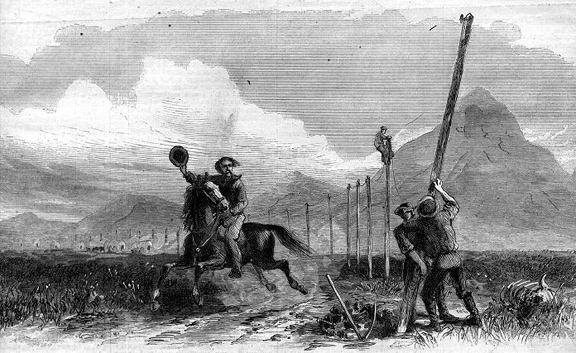
\includegraphics[width = 0.6\textwidth]{PoleA1}
        \caption{As primeiras linhas de telégrafo a serem construídas nos Estados Unidos \cite{polea1}.}
        \label{fig:polea1}
    \end{figure}
\end{frame}

\begin{frame}{Primeiro \textit{jamming} de rádio}
    \begin{minipage}[c]{0.6\linewidth}
        \begin{itemize}
            \item Com o aparecimento de sistemas de comunicação de rádio apareceu o \jamming{} intencional.
            \pause
            \item Numa corrida de iates da \textit{America's Cup}, um iate utilizou um transmissor mais potente para transmitir informação à imprensa para maior atenção e lucro.
            \item Foi a primeira instância de \jamming{} conhecida.
        \end{itemize}
    \end{minipage}
    \begin{minipage}[c]{0.39\linewidth}
        \begin{figure}[]
            \centering
            \includegraphics[width = \linewidth]{yachtrace}
            \caption{Corridas de iates americanos testemunharam o primeiro \jamming{} de rádio \cite{earlyradio}.}
            \label{fig:yachtrace}
        \end{figure}
    \end{minipage}
\end{frame}

\begin{frame}{Implementação militar}
    \begin{itemize}
        \item<1-> Os primeiros usos de \jamming{} de rádio militar foram treinadas pelo Reino Unido em 1902 e pelos Estados Unidos em 1903.
        \item<2-> As primeiras aplicações ocorreram na marinha.
        \item<3-> A guerra Russo-Japonesa entre 1904 e 1905 teve o primeiro grande uso de \jamming{} militar.
        \begin{itemize}
            \item Foi a primeira grande guerra onde ambas as partes utilizavam rádio para comunicações.
        \end{itemize}
    \end{itemize}
\end{frame}

\begin{frame}{Primeira Guerra Mundial}
    \begin{itemize}
        \item Comunicação por rádio na guerra manteve-se bastante primitiva.
        \item O pouco treino e hábito dos sistemas levou a pouco uso eficiente de \jamming{}.
        \item Ocorria bastante \jamming{} acidental entre forças aliadas devido a demasiadas transmissões num espaço reduzido.
    \end{itemize}
    \begin{figure}
        \centering
        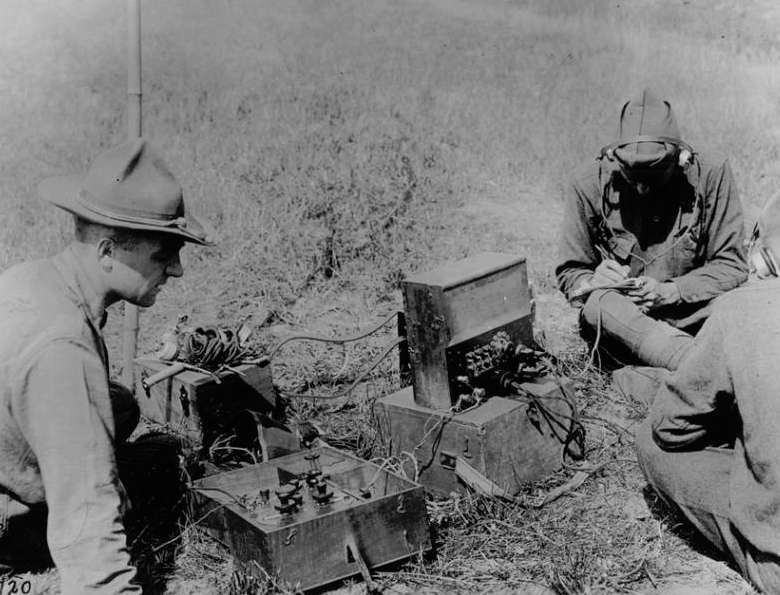
\includegraphics[width = 0.4\textwidth]{ww1}
        \caption{Primeiros aparelhos de rádio usados na Primeira Guerra Mundial \cite{worldwar1}.}
        \label{fig:ww1}
    \end{figure}
\end{frame}

\begin{frame}{Período Entre Guerras}
    No período após a Primeira Guerra Mundial, o potencial do rádio foi percebido e o desenvolvimento rápido.
    \begin{itemize}
        \item Transmissores diminuíram de tamanho e peso;
        \pause
        \item A sua performance melhorou;
        \pause
        \item A educação da população aumentou.
    \end{itemize}
    \pause
    Estes fenómenos levaram a uma melhoria dos sistemas de comunicação entre terra, mar e ar.
\end{frame}

\begin{frame}{Radar}
    Este período também viu o surgimento do radar.
    \begin{itemize}
        \item<1-> No início dos anos 1930, os radares conseguiam detetar alvos a 30 quilómetros.
        \item<2-> No fim da década, os radares aumentavam os seus alcances para mais de 160 quilómetros.
        \begin{itemize}
            \item O fator principal tornava-se a curvatura da Terra.
        \end{itemize}
        \item<3-> Também começavam a correr testes de \jamming{} de radar.
    \end{itemize}
    \begin{figure}
        \centering
        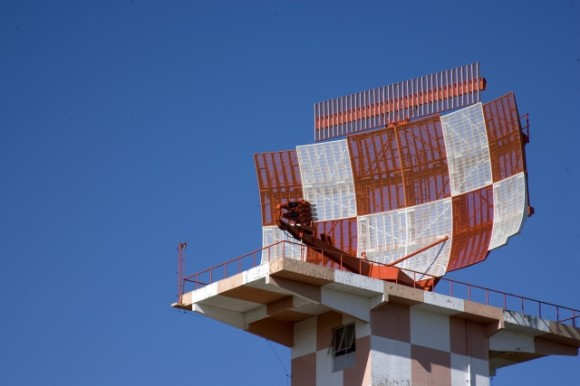
\includegraphics[width = 0.4\textwidth]{radarlisboa}
        \caption{Um transmissor-recetor de radar \cite{radarlisboa}.}
        \label{fig:radarlisboa}
    \end{figure}
\end{frame}

%\begin{frame}{Radar}
%    Por esta altura, o estudo de \jamming{} de radar foi cada vez mais desenvolvido.
%    \begin{itemize}
%        \item Os primeiros testes de tecnologias de \jamming{} começavam a ocorrer pela Europa, com os primeiros a serem feitos pela marinha inglesa em Londres.
%    \end{itemize}
%\end{frame}

\begin{frame}{Segunda Guerra Mundial}
    O rádio e os radares eram cada vez mais utilizados pelas forças armadas dos países europeus.
    \begin{itemize}
        \item A paragem de comunicação do inimigo teria cada vez mais importância no cenário da guerra.
        \item Rapidamente, a guerra tornou-se numa guerra de contra-medidas e contra-contra-medidas.
    \end{itemize}
\end{frame}

\begin{frame}{\textit{Battle Of The Beams}}
    Um cenário que ilustra esta natureza da guerra eletrónica é o período do \textit{Battle Of The Beams} entre a Alemanha e o Reino Unido.
    \begin{itemize}
        \item A Alemanha fez extensivo uso de radares para voar no escuro.
        \item Os radares utilizados serviam como um sistema de navegação primitivo.
        \item As forças aliadas foram apanhadas desprevenidas por bombardeamentos noturnos.
    \end{itemize}
\end{frame}

\begin{frame}{\textit{Knickebein}}
    A primeira fase deste período viu os alemães utilizarem uma variante do radar Lorenz.
    \begin{itemize}
        \item<1-> Este radar utiliza dois feixes para alinhar um avião com uma pista de aterragem.
        \item<2-> Os feixes apresentam características diferentes.
        \item<3-> Isto permite o piloto aterrar com segurança.
    \end{itemize}
    \begin{figure}
        \centering
        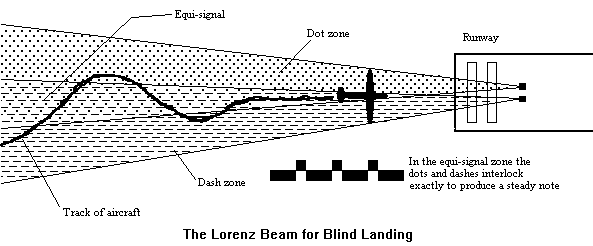
\includegraphics[width = 0.8\textwidth,trim = {0 8mm 0 0}, clip]{lorenz}
        \caption{Funcionamento do radar Lorenz \cite{pentagonknickebein}.}
        \label{fig:radarlisboa}
    \end{figure}
\end{frame}

\begin{frame}{\textit{Knickebein}}
    \begin{minipage}[c]{0.55\linewidth}
        \begin{itemize}
            \item<1-> Os dois radares foram utilizados pelos alemães para encontrar o alvo.
            \item<2-> Os britânicos redireccionaram os feixes de radar e emitiram réplicas próprias para desorientar os pilotos alemães.
            \item<3-> Isto causou despistes alemães e alguns pilotos até aterraram em solo inglês pensando que era a Alemanha.
        \end{itemize}
    \end{minipage}
    \hfill
    \begin{minipage}[c]{0.44\linewidth}
        \begin{figure}
            \centering
            {\tiny \includesvg[width = \textwidth]{Knickebein}}
            \caption{Mapa do uso do \textit{Knickebein} nos bombeamentos em Derby.}
        \end{figure}
    \end{minipage}
\end{frame}

\begin{frame}{Desenvolvimentos seguintes}
    \begin{itemize}
        \item As forças alemães desenvolveram novos sistemas de navegação via radar para combater a intervenção dos ingleses.
        \item Isto levou ao desenvolvimento dos radares \textit{X-Gerät} e mais tarde \textit{Y-Gerät}.
        \item A captura de aviões contendo esta tecnologia permitiu às forças inglesas bloquear as frequências utilizadas e impedir o uso destes radares.
        \item Este período terminou quando a força aérea alemã divergiu a sua atenção para a frente soviética.
        \item A \textit{Battle Of The Beams} ilustrou a natureza ataque-contra-ataque da guerra eletrónica.
    \end{itemize}
\end{frame}

\begin{frame}{Fim da Segunda Guerra Mundial}
    O fim da Segunda Guerra Mundial também viu o desenvolvimento e adopção de \textit{chaff}.
    \begin{figure}
        \centering
        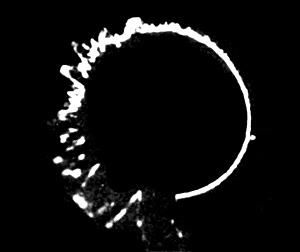
\includegraphics[width = 0.4\textwidth]{chaff}
        \caption{Exemplo de \textit{chaff} num \textit{display} de radar.}
    \end{figure}
    O uso de guerra eletrónica na frente do Pacífico também viu o uso de bastante \jamming{}, mas pouco desenvolvimento.
\end{frame}

\begin{frame}{Pós-Guerra}
    \begin{itemize}
        \item<1-> O período do pós-guerra viu muitas nações a considerarem a relevância do radar no campo de batalha.
        \item<2-> Começaram a ser definidos departamentos e oficiais dedicados à guerra eletrónica.
        \item<3-> Este período também viu o aparecimento primitivo do sector de \textbf{stealth}, o desenvolvimento de tecnologia para evitar deteção por radares anti-aéreos.
        \item<4-> O primeiro míssil auto-guiado \textit{surface-to-air} foi desenvolvido neste período inicial.
        \begin{itemize}
            \item Este levou ao desenvolvimento dos primeiros sistemas de \jamming{} de mísseis.
        \end{itemize}
    \end{itemize}
\end{frame}

\begin{frame}{Início da Guerra Fria}
    \begin{itemize}
        \item O início da guerra fria viu o confronto de inteligência entre os Estados Unidos da América e a União Soviética.
        \item Embora não houvesse confronto direto, ambas as partes faziam missões para obtenção de inteligência no inimigo.
        \item Com o risco de descoberta ser poder levar a resposta aprontada do inimigo, as missões eram realizadas com discreção extrema.
        \item Este período viu um investimento em tecnologia de obtenção de inteligência.
    \end{itemize}
\end{frame}

\begin{frame}{Missões ELINT}
    \begin{minipage}[c]{0.57\textwidth}
        \begin{itemize}
            \item As missões de obtenção de inteligência electrónica dos Estados Unidos começaram por esta altura.
            \item Utilizando aeronaves como o \textit{Lockheed U-2} obtiam informações sobre radares e sistemas de comunicação da União Soviética evitando deteção. Informações como
            \begin{itemize}
                \item Frequência de pulsação;
                \item Intervalo de tempo;
                \item Velocidade de \textit{scanning};
                \item Direcção de \textit{scanning};
                \item Localização de radares.
            \end{itemize}
        \end{itemize}
    \end{minipage}
    \hfill
    \begin{minipage}[c]{0.4\textwidth}
        \begin{figure}
            \centering
            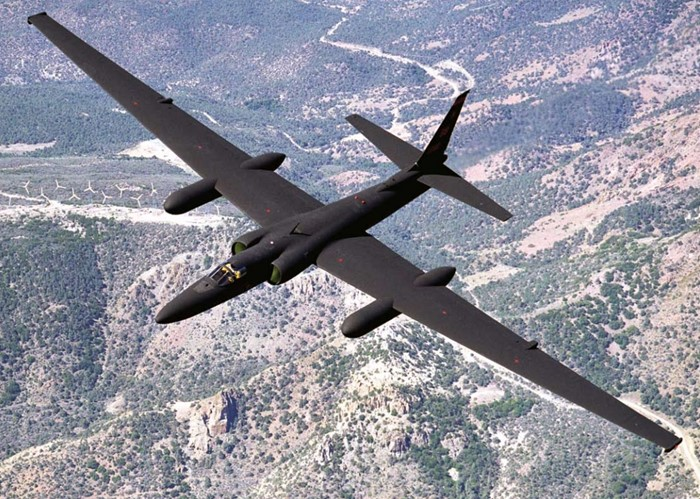
\includegraphics[width = \textwidth]{lockheedu2}
            \caption{O \textit{Lockheed U-2} utilizado pelos Estados Unidos.}
        \end{figure}
    \end{minipage}
    \vspace*{5mm}
    
    As missões terminaram quando um avião foi alvejado após detecção por tecnologia nova da União Soviética.
\end{frame}

\begin{frame}{A Guerra do Vietname}
    \begin{itemize}
        \item O envolvimento dos Estados Unidos na guerra do Vietname implicou um grande progresso na evolução.
        \begin{itemize}
            \item A grande quantidade de baixas sofridas devido a armamentos anti-aéreos levou ao estudo de armamento anti-radar.
        \end{itemize}
    \end{itemize}
\end{frame}

\begin{frame}{Os \textit{Wild Weasels}}
    \begin{minipage}[c]{0.44\textwidth}
        \begin{figure}
            \centering
            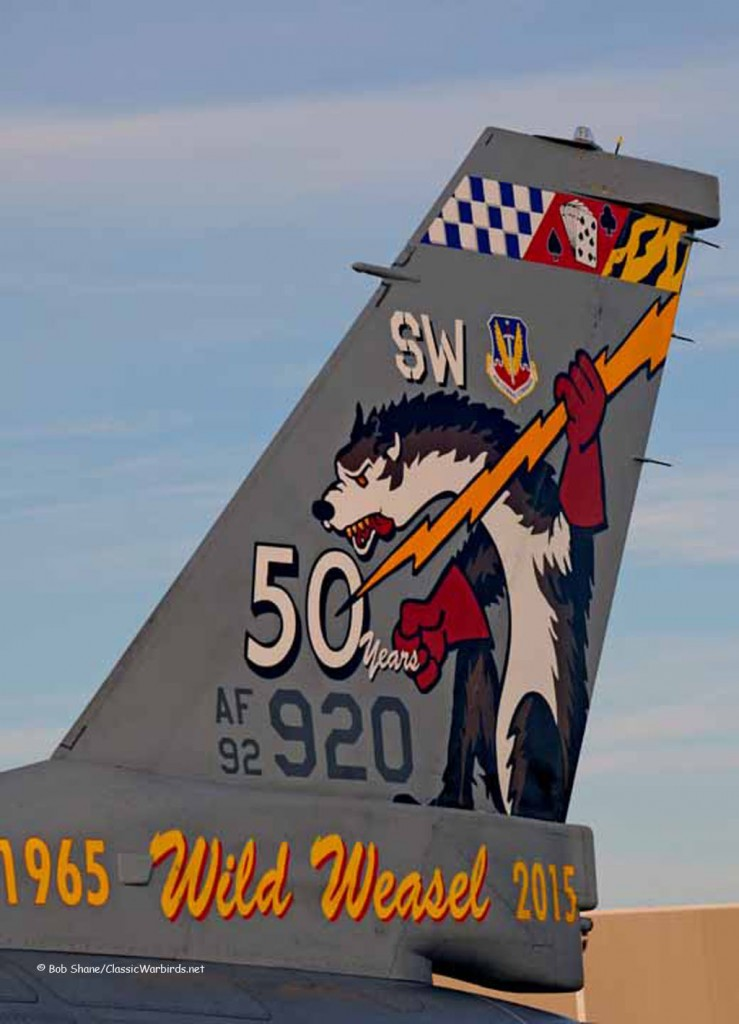
\includegraphics[width=0.9\textwidth]{wildweasel}
            \caption{A cauda de um F-16 \textit{Wild Weasel}.}
        \end{figure}
    \end{minipage}
    \hfill
    \begin{minipage}[c]{0.55\textwidth}
        \begin{itemize}
            \item Aviões começaram a ser equipados com mísseis que seguem sinais de radares, para destruir zonas mais fortificadas.
            \item Estes aviões foram denominados \textit{Wild Weasels}, que escoltavam aviões de artilharia pesada e protegiam-nos dos armamentos anti-aéreos terrestres.
            \item Esta combinação possibilitou o domínio aéreo e a invasão de zonas fortificadas nos terrenos vietnamitas.
        \end{itemize}
    \end{minipage}
\end{frame}

\begin{frame}{Guerra do Golfo}
    A guerra no Golfo Persa em 1990 e 1991 iniciou a era moderna da guerra eletrónica.
    \begin{itemize}
        \item As forças da coalição concentraram o seu poder de fogo nas estruturas de comunicação, deteção e armamento anti-aéreo para debilitar a força eletrónica do exército iraquiano.
        \item Rapidamente se criou um domínio aéreo sobre a região que acabou por decidir o resultado da guerra.
    \end{itemize}
\end{frame}

\begin{frame}{Inovações da Guerra do Golfo}
    A guerra trouxe várias tecnologias de guerra eletrónica para o campo de batalha.
    \begin{itemize}
        \item Reunião de inteligência foi feita por aviões \textit{stealth}, indetetáveis ao radar inimigo.
        \item A utilização de \textit{decoys} afetou a deteção dos radares e permitiu a entrada de artilharia aérea pesada sem perigo.
        \item A destruição de radares facilitou a invasão de tropas terrestres.
    \end{itemize}
    \begin{figure}
        \centering
        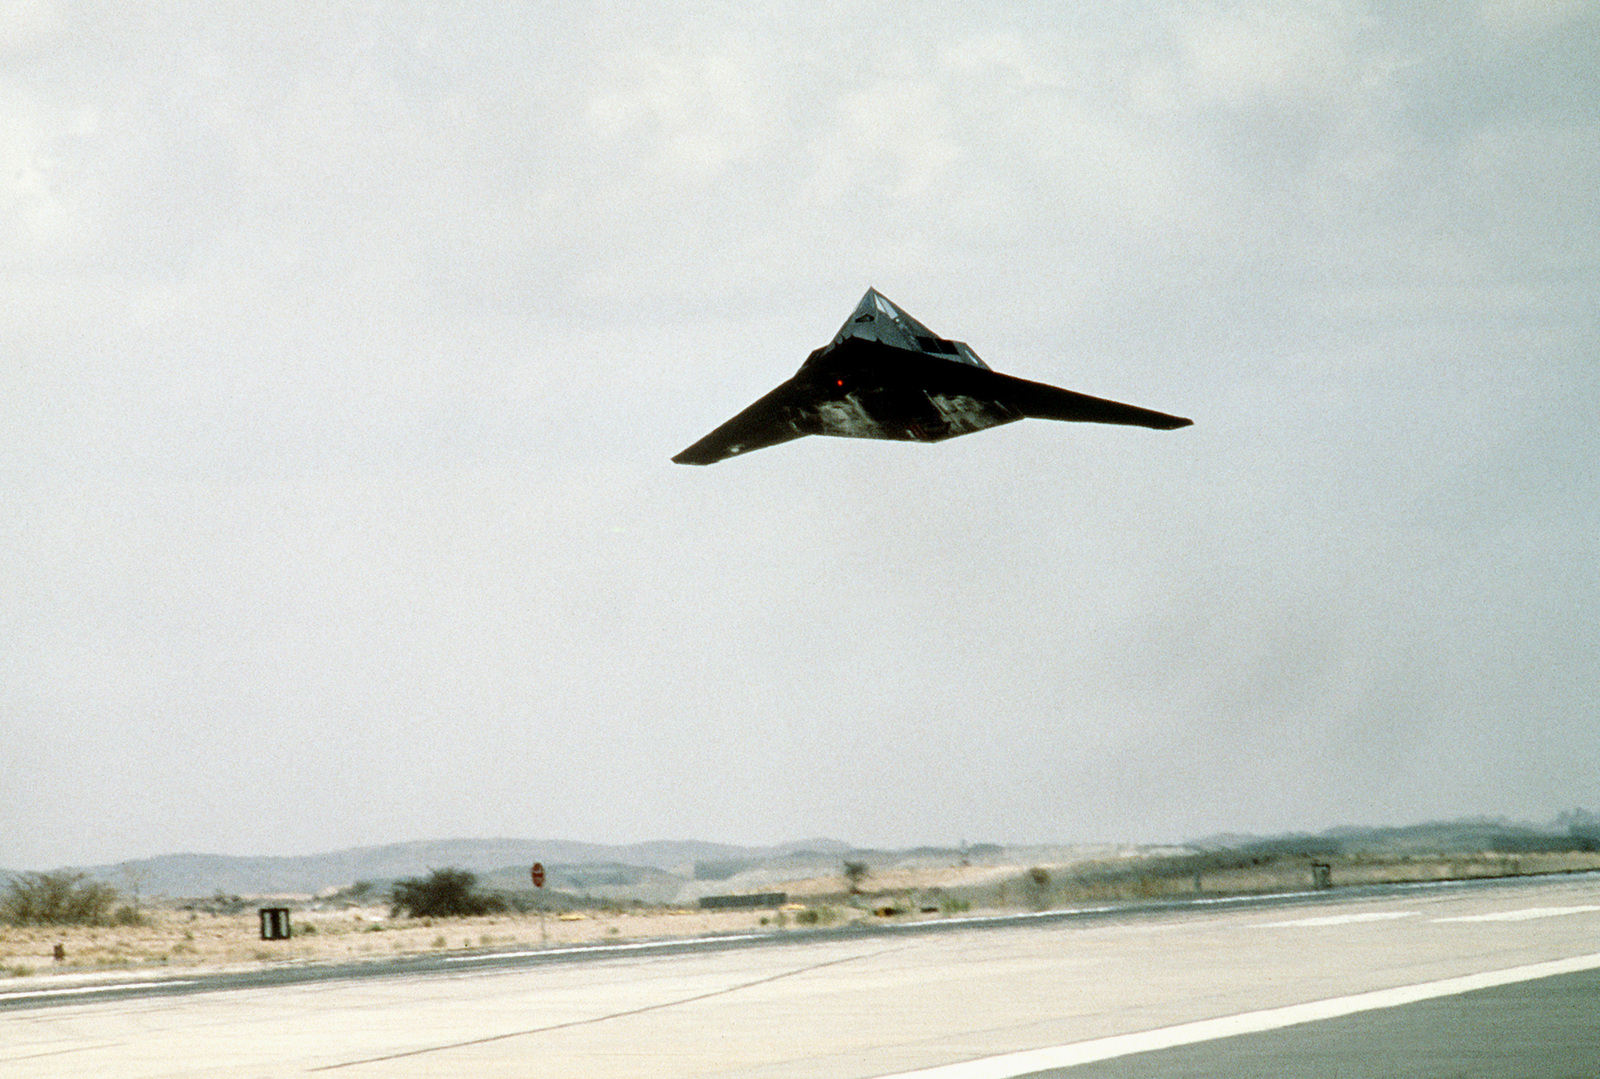
\includegraphics[width = 0.4\textwidth]{f117}
        \caption{Um \textit{Lockheed F-117 Nighthawk}, um avião \textit{stealth} utilizado extensivamente na guerra.}
    \end{figure}
\end{frame}

%----------------Pedro starts here ---------------------%


\section{Ataque Eletrónico}

\begin{frame}{Ataque Electrónico (AE) - Jamming }
    \begin{itemize}
        \item Mudando as características elétricas e magnéticas do ambiente;
        \vspace*{3mm}
        \item  Reduzindo a detectibilidade no radar e detectibilidade térmica da aeronave; 
        \vspace*{3mm}
        \item Nos dias actuais, o significado básico de ataque electrónico é o uso de vários sinais Jamming que afectam directamente os sistemas electrónicos na banda de radio frequência.
    
    \end{itemize}
    
   
\end{frame}

\begin{frame}{Ataque Electrónico (AE) - Jamming}
    
    Jammer constítuido por: 
     \vspace*{5mm}
    \begin{itemize}
        \item Sistemas de controlo e suporte;
        \vspace*{3mm}
        \item  Um subsistema que produz sinais de Jamming; 
        \vspace*{3mm}
        \item Amplificadores de alta frequência e geradores com moduladores;
         \vspace*{3mm}
         \item Dispositivos de Antena.
    
    \end{itemize}
    
   
\end{frame}


\begin{frame}{Jammer automático}
    
\begin{figure}[ht]
\centering
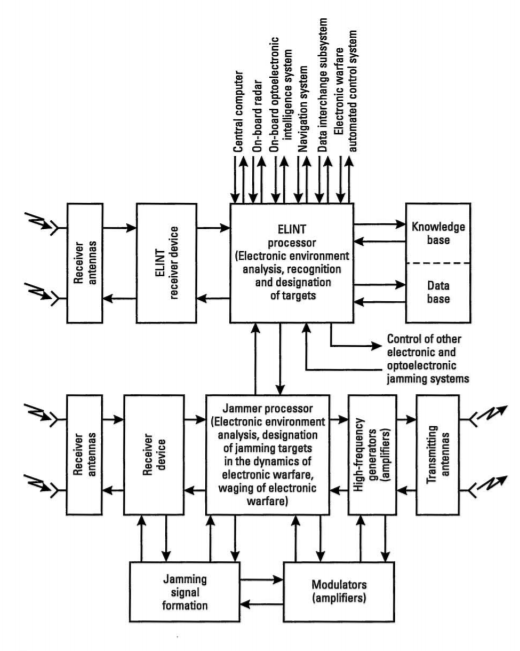
\includegraphics[width=0.4\textwidth]{jam1.png}
\caption{Diagrama de blocos para um Jammer automático}
\label{jam1}
\end{figure} 
\end{frame}



\begin{frame}{Jamming}
    
    Tipos de Jamming:
      \vspace*{5mm}
    \begin{itemize}
        \item Destrutivo;
        \vspace*{3mm}
        \item  Dissimulação; 
        \vspace*{3mm}
        \item Ilusão.
    
    \end{itemize}
    
   
\end{frame}



\begin{frame}{Jamming destrutivo }
    
      \vspace*{5mm}
    \begin{itemize}
    \item Potência da emissão de Jamming \begin{equation*}
P_{rec}= \frac{P_j G_j}{4 \pi D_j ^2} A_{rec} \gamma_j \eta_j    
\end{equation*}

\item Gama dinâmica limitada de receptores 
\begin{equation*}
K_{drr}= \frac{P_{rec max}}{P_{rec min}}    
\end{equation*}
$P_{rec min}$- limite de sensibilidade , $D_j$ - distância do jammer ao alvo, $K_{drr}$ - gama dinâmica do receptor  $P_{rec max}$ - Potência radiada requerida para causar uma sobrecarga dinâmica
    \end{itemize}
    
  \end{frame}




\begin{frame}{Ataque Electrónico (AE) - Jamming}\Large
    
    
      \vspace*{5mm}
    \begin{itemize}
        \item Nível táctico - Destruição das defesas Anti-Aéreas num ataque;
        \vspace*{6mm}
        \item  Nível Operacional - Simular dano nas defesas de forma a criar uma ilusão ao inimigo que realiza um ataque.
        \vspace*{3mm}
     
    
    \end{itemize}
    \end{frame}

\begin{frame}{Jamming}
    \begin{figure}[ht]
        \begin{minipage}[c]{0.49\linewidth}
            \centering
            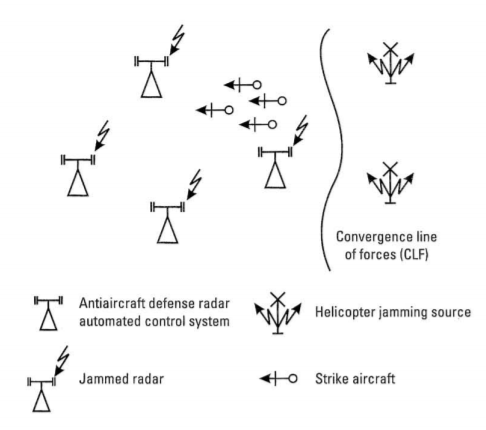
\includegraphics[width=50mm]{jam2.png}
            \caption{Métodos de ocultação de aviões (helicópteros) e outros alvos de áreas fixas usando jamming}
            \label{jam2}
        \end{minipage}
        \hspace{\fill}
        \begin{minipage}[c]{0.49\linewidth}
            \centering
            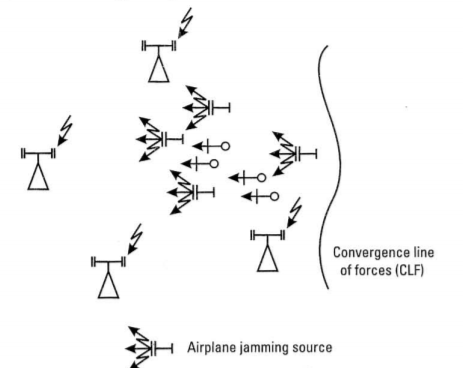
\includegraphics[width=50mm]{jam3.png}
            \caption{Métodos de ocultação de aviões em formação de batalha usando jamming.}
            \label{jam3}
        \end{minipage}
    \end{figure}
\end{frame}



\section{Protecção Electrónica}

%----------------Manito starts here ---------------------%
% para passar ha que pagar portagem que até se lixam...
\begin{frame}{Protecção Electrónica (PE)}
    \begin{itemize}
        \item Negar o efeito do jamming inimigo, mantendo capacidades operacionais aliadas;
        \vspace*{3mm}
        \item Ciclo contínuo de AE $\Rightarrow$ PE $\Rightarrow$ AE
        \vspace*{3mm}
        \item Vários métodos em uso, entre eles:
        \begin{itemize}
            \item Compressão de pulso
            \item Espectro de difusão em frequência variável
            \item Anulamento de lóbulo secundário
            \item Polarização
            \item Chaff
            \item Direccionamento por radiação
        \end{itemize}
    \end{itemize}
\end{frame}

\begin{frame}{Compressão de pulso}
    Exemplo: Radar de pulso
    \begin{itemize}
        \item<1-> Pulso sinusoidal de período T
        \item<1-> $SNR = \frac{K^2 A^2 T}{\sigma^2}$
        \item<1-> $\Delta R = \frac{1}{2} c \Delta T$
        \item<1-> Como reduzir efeitos de \textit{jamming}?
        \begin{itemize}
            \item<2-> Aumento do período do pulso
            \item<2-> Maior SNR
            \item<2-> Aumento da energia, diminuição da resolução de distância
        \end{itemize}
    \end{itemize}
\begin{figure}[ht]
\centering
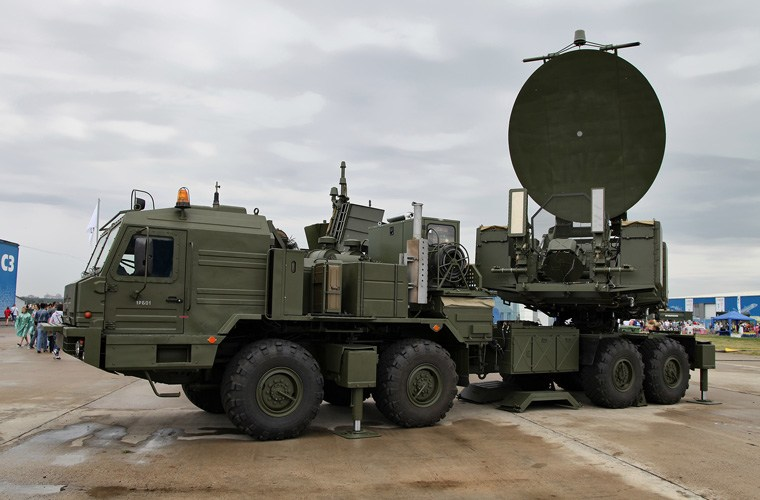
\includegraphics[width=0.4\textwidth]{graphics/jammer_militar.jpg}
\caption{\textit{Jammer} militar Krasukha-2}
\label{jammer_militar}
\end{figure}
\end{frame}

\begin{frame}{Compressão de pulso}
    Modulação linear em frequência do pulso - \textit{chirping}
    \begin{itemize}
        \item<1-> Modulação em torno da frequência da portadora, $f_0$
        \item<1-> Banda de modulação $\Delta f$
        \item<2-> Correlação centrada em $t=0$, aproximadamente função \textit{sinc}
        
    \end{itemize}
    \begin{figure}[ht]
\centering
\includegraphics[width=0.4\textwidth]{graphics/modulaçao_chirp.jpg}
\caption{Modulação do pulso em frequência - \textit{chirping}}
\label{modulacao_chirp}
\end{figure}
\end{frame}

\begin{frame}{Compressão de pulso}
 Modulação linear em frequência do pulso - \textit{chirping}
    \begin{itemize}
    \item Duração do pulso: $T' = \frac{1}{\Delta f}$
    \item Para certos valores de $\Delta t$, $T \ge T'$ $\Rightarrow$ compressão
    \item Relação entre potências: $P' = P \times \frac{T}{T'}$
    \end{itemize}

\begin{figure}[ht]
\centering
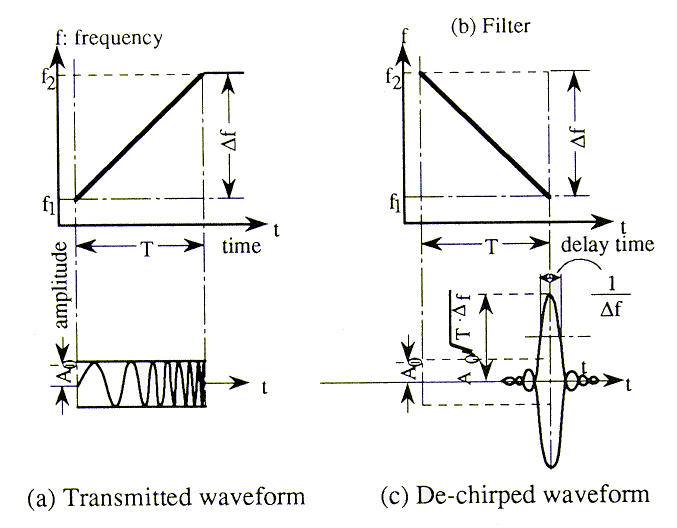
\includegraphics[width=0.4\textwidth]{graphics/chirped_result.PNG}
\caption{Pulso e sinal de eco desmodulado}
\label{chirped_result}
\end{figure}
\end{frame}


\begin{frame}{Espectro de difusão em frequência variável}
    \begin{itemize}
    \item Mudança da frequência de operação ao longo do tempo;
    \item Sincronia usando códigos pseudoaleatórios
    \end{itemize}
    \begin{figure}[ht]
\centering
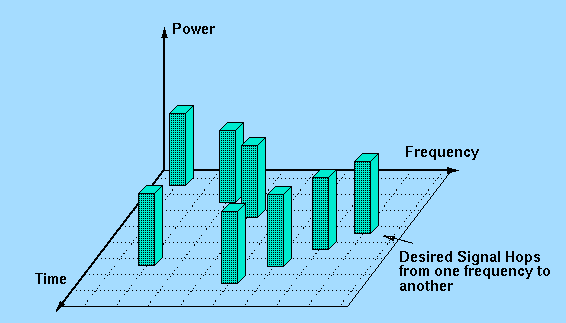
\includegraphics[width=0.4\textwidth]{graphics/frequency_hopping.png}
\caption{Exemplo de variação da frequência no tempo}
\label{frequency_hopping}
\end{figure}
\end{frame}
    
\begin{frame}{Espectro de difusão em frequência variável}
    \begin{itemize}
    \item \textit{Jammers} necessitam de cobrir um espectro de frequências maior
    \item Menos potência de transmissão disponível para frequências específicas
    \item Redução da capacidade de \textit{jamming} dos sinais
    \end{itemize}
    \begin{figure}[ht]
\centering
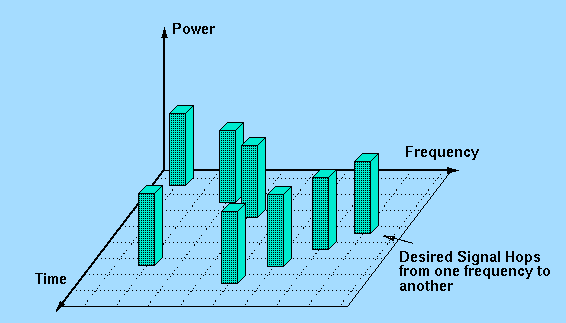
\includegraphics[width=0.4\textwidth]{graphics/frequency_hopping.png}
\caption{Exemplo de variação da frequência no tempo}
\label{frequency_hopping}
\end{figure}
\end{frame}

\begin{frame}{Anulamento de lóbulo secundário}
    \begin{itemize}
    \item<1-> Antenas direccionais apresentam padrões de radiação com lóbulos secundários
    \item<2-> Potencial de \textit{jamming}
    \item<3-> Redução da capacidade de \textit{jamming} dos sinais
    \end{itemize}
    \begin{figure}[ht]
\centering
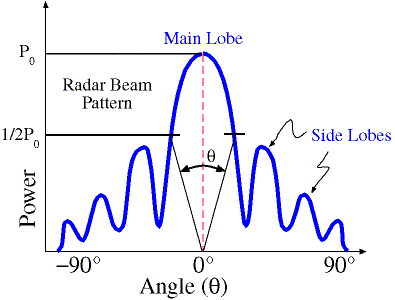
\includegraphics[width=0.4\textwidth]{graphics/radar_antenna_lobes.png}
\caption{Padrão de radiação de uma antena de radar}
\label{radiation_pattern}
\end{figure}
\end{frame}

\begin{frame}{Anulamento de lóbulo secundário}
Solução: Utilização de uma antena secundária omnidireccional
    \begin{itemize}
    \item<1-> Ganho do receptor secundário superior ao ganho dos lobulos secundários
    \item<2-> Comparação de intensidades de sinal
    \item<3-> Receptor secundário com sinal superior à antena principal $\Rightarrow$ lobulos secundários em recepção
    \item<4-> Minimização significativa de sinais fora do eixo da antena
    \end{itemize}
    \begin{figure}[ht]
\centering
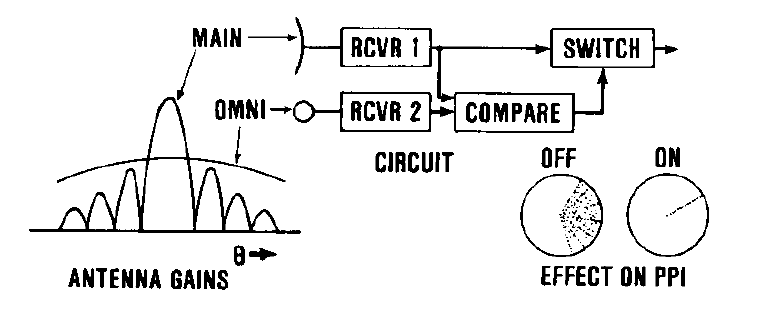
\includegraphics[width=0.4\textwidth]{graphics/sidelobe_suppresion.png}
\caption{Esquema de funcionamento de anulamento de lóbulo secundário}
\label{sidelobe_suppression}
\end{figure}
\end{frame}

\begin{frame}{Polarização}
    \begin{itemize}
    \item<1-> Ondas transmitidas são polarizadas
    \item<2-> Necessário igualar polarizações para recepção óptima
    \end{itemize}
    \begin{figure}[ht]
\centering
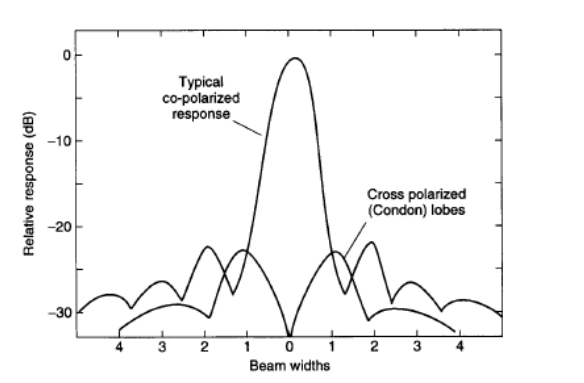
\includegraphics[width=0.4\textwidth]{graphics/parabolic_polarization_response.png}
\caption{Resposta de uma antena parabólica a ondas polarizadas}
\label{sidelobe_suppression}
\end{figure}
\end{frame}

\begin{frame}{Polarização}
\textit{Jammer} com uma única polarização
    \begin{itemize}
    \item<1-> Solução simples: duas antenas com polarizações diferentes
    \item<2-> Apenas uma das antenas recebe interferência
    \end{itemize}
    \begin{figure}[ht]
\centering
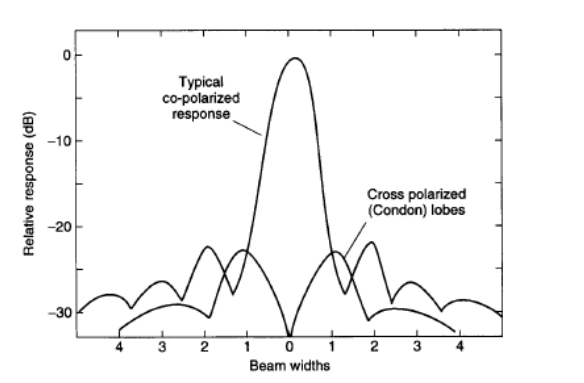
\includegraphics[width=0.4\textwidth]{graphics/parabolic_polarization_response.png}
\caption{Resposta de uma antena parabólica a ondas polarizadas}
\label{sidelobe_suppression}
\end{figure}
\end{frame}

\begin{frame}{\textit{Chaff}}
    \begin{itemize}
    \item<1-> Pequenas peças de metal espalhadas no ar
    \item<2-> Antenas de meio dipolo
    \item<3-> Método antigo mas eficaz
    \end{itemize}
    \begin{figure}[ht]
\centering
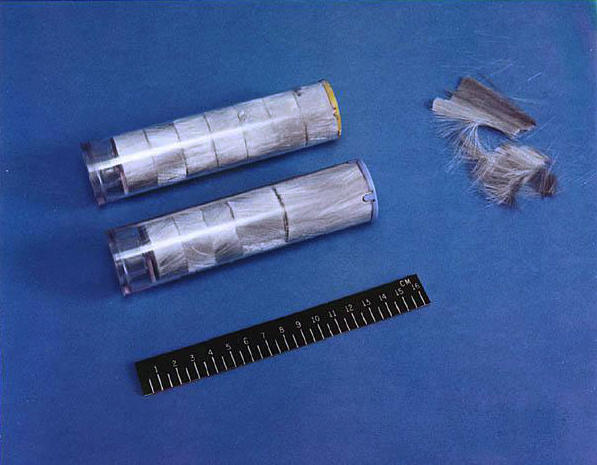
\includegraphics[width=0.4\textwidth]{graphics/Usnchaff.jpg}
\caption{\textit{Chaff} moderno}
\label{chaff_photo}
\end{figure}
\end{frame}

\begin{frame}{\textit{Chaff}}
    \begin{itemize}
    \item<1-> Cria ecos de radar quando iluminado
    \item<2-> Curta duração
    \item<3-> Permite mascarar aeronave de misseis, artilharia terrestre e outras aeronaves
    \end{itemize}
    \begin{figure}[ht]
\centering
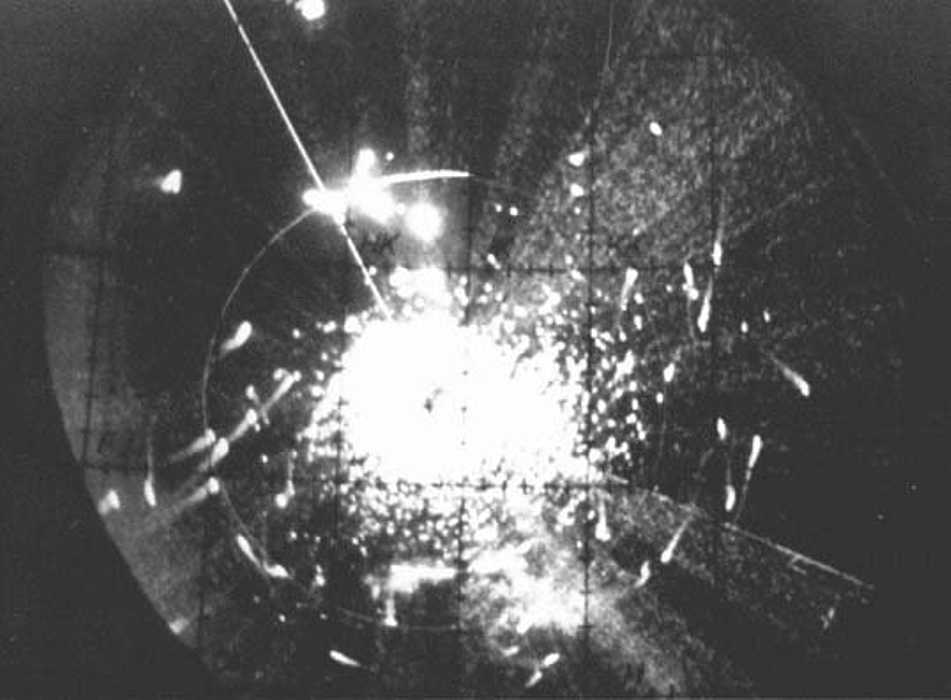
\includegraphics[width=0.4\textwidth]{graphics/chaff_radarjpg.jpg}
\caption{Eco de radar devido a uma núvem de \textit{Chaff}}
\label{chaff_cloud_echo}
\end{figure}
\end{frame}

\begin{frame}{Direccionamento por radiação}
Usar sinais de \textit{jamming} contra eles mesmos
    \begin{itemize}
    \item<1-> Detecção da localização de um sistema de \textit{jamming} usando a radiação deste
    \item<2-> Direccionamento de míssil contra a fonte de radiação
    \item<3-> Exemplo: usando supressão de lóbulo lateral
    \begin{itemize}
        \item Detecção do sinal de \textit{jamming}
        \item Determinação do ângulo de chegada do sinal
        \item \textit{Lock-on} do míssil para a fonte da radiação
    \end{itemize}
    \end{itemize}
    \begin{figure}[ht]
\centering
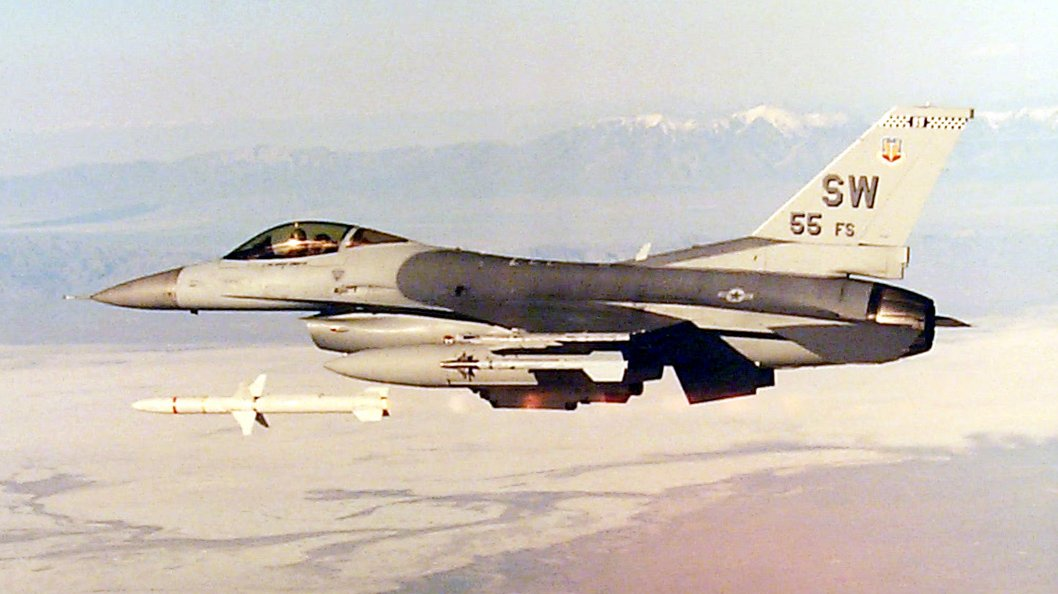
\includegraphics[width=0.4\textwidth]{graphics/arm_missile.jpg}
\caption{Míssil anti-radiação (ARM) AGM-88 HARM}
\label{arm_missile}
\end{figure}
\end{frame}

\section{Suporte Electrónico de Guerra}
%----- Suporte electrónico de guerra -----%    
    
    \begin{frame}{Suporte Electrónico de Guerra - Localização do alvo}
   
    \begin{itemize}
        \item Sabendo a localização dos alvos, indica-nos a disposição das forças;
       
        \item Pode dar uma indicação do tipo de entidade numa localização particular, agrupando diferentes tipos de emissores.
        
    \end{itemize}
    \begin{figure}[ht]
\centering
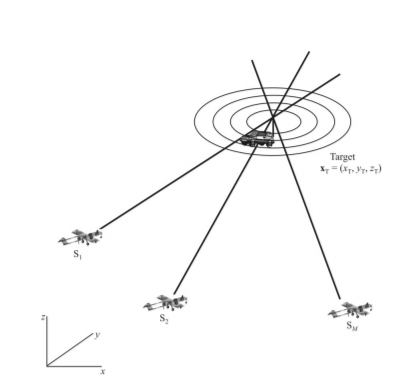
\includegraphics[width=50mm]{target1.png}
\caption{Intersecção das linha de direcção medidas - \textit{Line of Bearing}}
\label{target1}
\end{figure}
\end{frame}

\begin{frame}{Suporte Electrónico de Guerra - Triangulação}
   
    \begin{itemize}
        \item Pode ser implementada numa variedade de plataformas (aviões);
       
        \item Requer um aglomerado de Antenas; 
        
        \item Fornece métodos para estimar o azimute dos ângulos de chegada dos sinais com base na medição da diferença de tempo de chegada ou diferença de fase dos sinais em duas antenas espaçadas a metade (ou menos) do comprimento de onda do sinal.
        
    \end{itemize}
    \begin{figure}[ht]
\centering
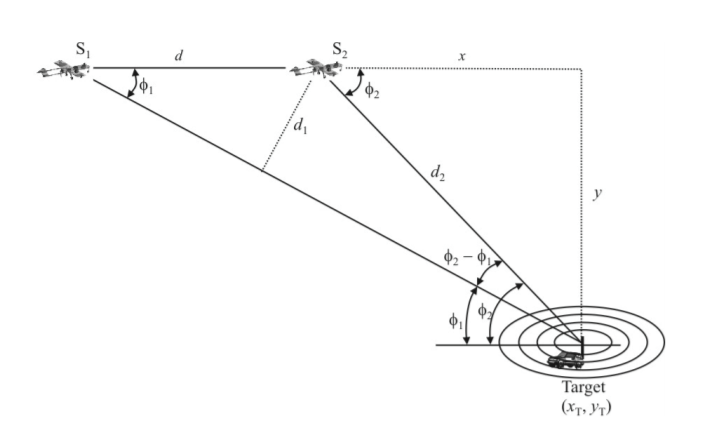
\includegraphics[width=70mm]{target4.png}
\caption{Relações Geométricas para o Ponto Fixo pela triangulação}
\label{target4}
\end{figure}
\end{frame}

\begin{frame}{Suporte Electrónico de Guerra - Triangulação}
   
    \begin{itemize}
        \item \begin{equation*}
    \sin{\phi_1} = \frac{d_1}{d} \Rightarrow 
    d_1 = d \sin{\phi_1}
    \end{equation*}


       
        \item \begin{equation*}
\sin{\phi_2 - \phi_1} = \frac{d_1}{d_2} \Rightarrow d_2 = \frac{d_1}{\sin{\phi_2 - \phi_1}} \Rightarrow d_2 = \frac{d \sin{\phi_1}}{\sin{\phi_2 - \phi_1}}     
\end{equation*}
        
        \item As distâncias para o alvo ao sensor $S_2$, $x$ and $y$, podem ser obtidas:

\begin{equation*}
x = d_2 \cos{\phi_2}     
\end{equation*}

\begin{equation*}
y = d_2 \sin{\phi_2}     
\end{equation*}
        
    \end{itemize}
    \begin{figure}[ht]
\centering
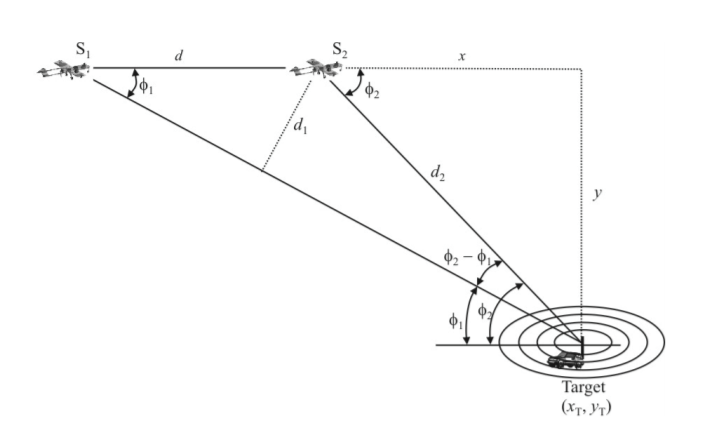
\includegraphics[width=40mm]{target4.png}
\caption{Relações Geométricas para o Ponto Fixo pela triangulação}
\label{target4}
\end{figure}
\end{frame}

  \begin{frame}{Suporte Electrónico de Guerra - Triangulação}
   
    \begin{itemize}
        \item Algoritmos disponíveis para o cálculo do Ponto fixo baseados nas técnicas de estimação do \textit{LSE};
      \vspace*{5mm}
        \item Estes princípios podem-se extender a 3 dimensões e ao uso de mais de 2 sensores. 
        \vspace*{5mm}
        \item Desenhar as linhas de direcções medidas e observar directamente onde se cruzam é outra técnica de triangulação. Os sensores podem ser apenas um a mover-se ou três estacionários, como mostra a figura \ref{target5}.
    \end{itemize}
\end{frame}
    
\begin{frame}{Suporte Electrónico de Guerra - Triangulação}
    \begin{figure}[ht]
        \begin{minipage}[b]{0.49\linewidth}
            \centering
            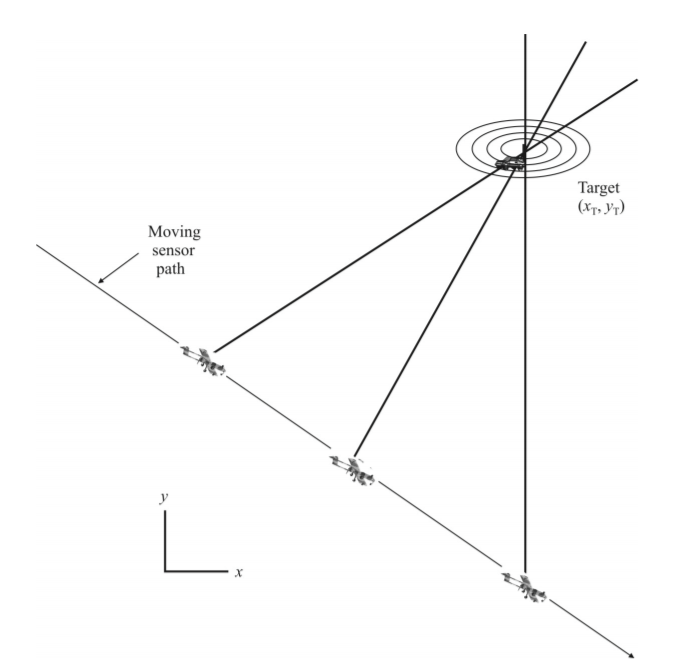
\includegraphics[width=50mm]{target5.png}
            \caption{Triangulação}
            \label{target5}
        \end{minipage}
        \hspace{\fill}
        \begin{minipage}[b]{0.49\linewidth}
            \centering
            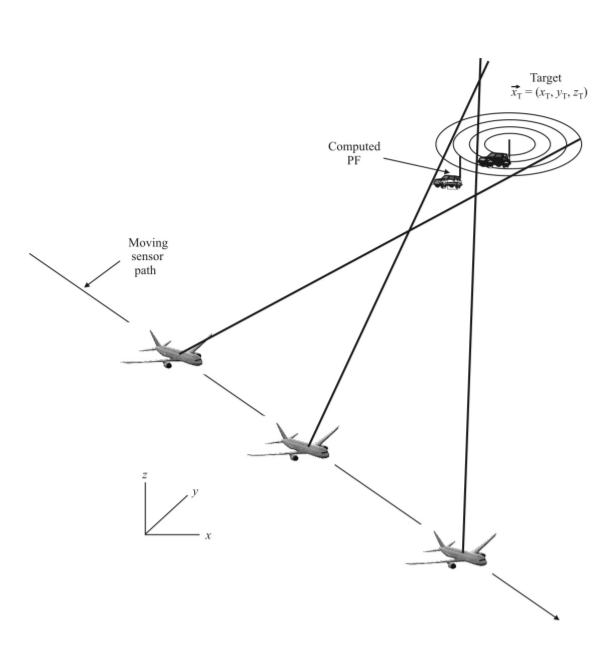
\includegraphics[width=50mm]{target6.png}
            \caption{Erros aleatórios no cálculo do Ponto Fixo}
            \label{target6}
        \end{minipage}
    \end{figure}
\end{frame}


\begin{frame}{Suporte Electrónico de Guerra - Triangulação}
   
    \begin{itemize}
        \item Em geral os sinais são corrompidos por erros de medição e ruído (Branco Gaussiano de zero de média);
      \vspace*{5mm}
        \item Se o ruído for aleatório, a linha de direcções medida poderá ser maior ou menor do que a actual, resultando na elipse de erro;
        \vspace*{5mm}
        \item Os sensores podem exibir \textit{bias}.
    \end{itemize}
\end{frame}

    \begin{frame}{Localização do alvo - Triangulação}
   
    \begin{itemize}
        \item Trêns métodos não estatísticos para estimar a localização do alvo dado um triângulos, figura \ref{target7} 
    \end{itemize}
    \begin{figure}[ht]
\centering
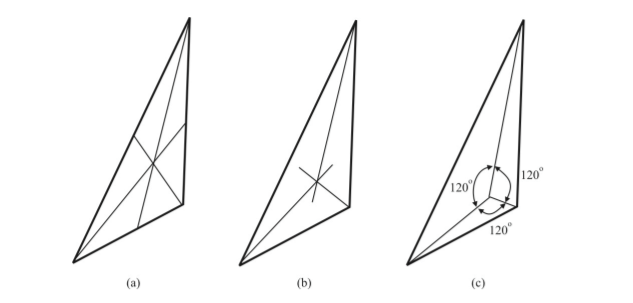
\includegraphics[width=70mm]{target7.png}
\caption{Cálculos de Ponto Fixo não estatísticos com só três linhas de direcção. (a) intersecção das médias (b) intersecção dos ângulos bissectores e (c) Ponto Steiner (definido pelo ponto onde os ângulos entre as linhas de direcção que vêm dos cantos são todas 120º). Todos eles são métodos para estimar o centroide do triângulo.}
\label{target7}
\end{figure}
\end{frame}

 \begin{frame}{Métodos de Optimização de localização do Ponto fixo}
   
    \begin{itemize}
        \item Baseados na minimização do erro entre o valor estimado e o Ponto Fixo;
         \vspace*{5mm}
        \item Generalizações do algoritmo da estimação dos mínimos quadrados. 
        \vspace*{5mm}
         \item Estimação total dos mínimos quadrados - permite a existência de ruído nas medições; 
        \vspace*{5mm}
        \item Estimação do Pesos dos Mínimos Quadrados - Matriz dos Pesos $\mathbf{W_k}\neq I $
         
    \end{itemize}
   
\end{frame}

  \begin{frame}{Triangulação - Métodos de Optimização}
   
    \begin{itemize}
  
        
        \item Estimação do Pesos dos Mínimos Quadrados - Matriz dos Pesos $\mathbf{W_k}\neq I $
       
        \vspace*{3mm}
        
        \item Algoritmo de triangulação dos Mínimos quadrados do Brown, figura \ref{target10}.
        
        
        
    \end{itemize}
    \begin{figure}[ht]
\centering
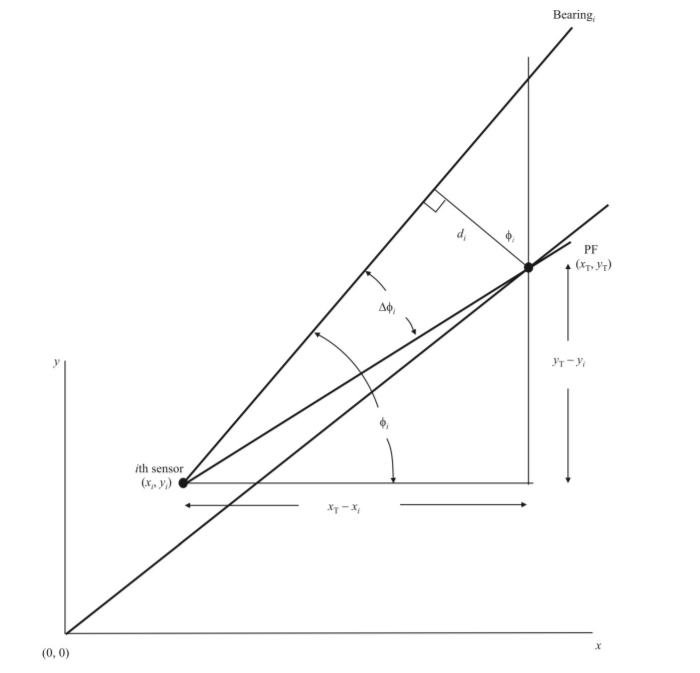
\includegraphics[width=60mm]{target10.png}
\caption{Definição dos termos de derivação do algoritmo do método dos mínimos quadrados de Brown}
\label{target10}
\end{figure}
\end{frame}


\begin{frame}{Triangulação - Métodos de Optimização}
   
    \begin{itemize}
 
        \item Algoritmo de Estimação do Erro dos mínimos quadrados Hemisférico - A medição da linha de direcção a partir de um sensor $\phi_i$ projectada na superficíe da Terra no hemisfério Norte
        
        \item \begin{equation*}
    \cos{\phi_i}= \frac{y_t - y_i}{\sqrt{(y_T - y_i)^2+(x_T - x_i)^2}}
\end{equation*}
       
    \end{itemize}
    \begin{figure}[ht]
\centering
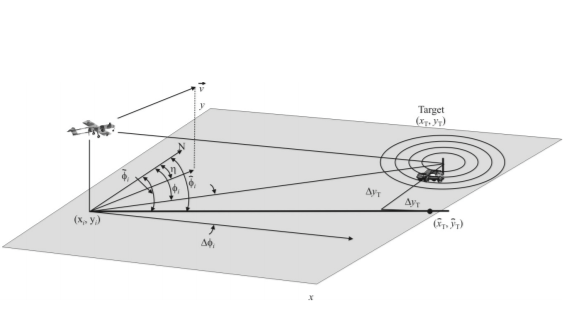
\includegraphics[width=60mm]{target11.png}
\caption{Geometria para o hemisférico calculado pelos mínimos quadrados}
\label{target11}
\end{figure}
\end{frame}


\begin{frame}{Triangulação - Métodos de Optimização}
   
    \begin{itemize}
 
        \item Algoritmos da Estimação Mínimos Quadrados Pages-Zamora baseado nos requisitos de telemóvel impostos pelo \textit{Federal Communications Committee} nos Estados Unidos da América.
        
        \item \begin{equation*}
    \Vec{d_0}= \Vec{d_{oi}+ d_i\Vec{v_i}} 
\end{equation*}

    \item \begin{equation*}
    x_T = x_i + d_{oi}\cos{\phi_i}
\end{equation*}
\begin{equation*}
    y_T = y_i + d_{oi}\sin{\phi_i}
\end{equation*}
       
    \end{itemize}
    \begin{figure}[ht]
\centering
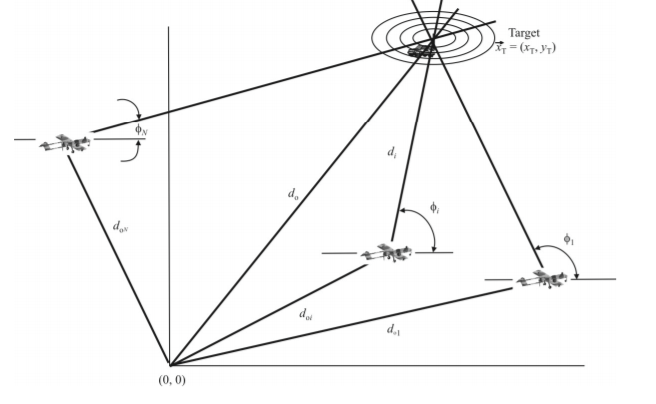
\includegraphics[width=75mm]{target12.png}
\caption{Geometria descritiva do algoritmo desenvolvido por Pages-Zamora.}
\label{target12}
\end{figure}
\end{frame}


\begin{frame}{Triangulação - Métodos de Optimização}
   
    \begin{itemize}
 
        \item Método da Estimação dos mínimos quadrados total - obtém-se elevando ao quadrado a equação do do método de Estimação dos minímos quadrados Hemisférico:
        \vspace{5mm}
        \item \begin{equation*}
    \cos{\phi_i}^2= \frac{(x_t - x_i)^2}{(y_T - y_i)^2+(x_T - x_i)^2}
\end{equation*}
       
    \end{itemize}
  \end{frame} 


\begin{frame}{Triangulação - Métodos de Optimização}
   
    \begin{itemize}
 
        \item O filtro de Kalman pode também ser aplicado na estimação do ponto fixo;
        
        \item No caso da aplicação filtro de Kalman padrão, os resultados são óptimos no método dos mínimos quadrados relativamente aos erros.
    
       
    \end{itemize}
    \begin{figure}[ht]
\centering
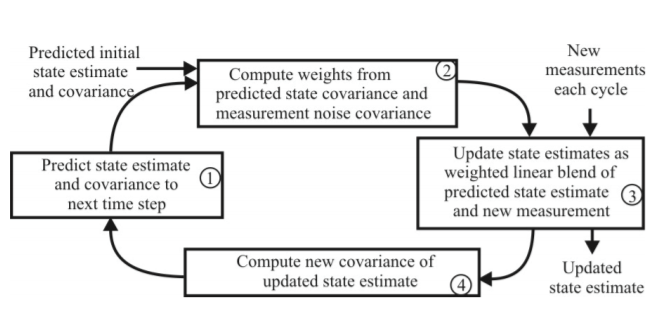
\includegraphics[width=95mm]{target2.png}
\caption{Algoritmo do filtro de Kalman}
\label{target2}
\end{figure}
\end{frame}

\begin{frame}{Triangulação - Métodos de Optimização}
   
    \begin{itemize}
 
        \item A Extenção do filtro de Kalman resulta na aplicação do filtro de Kalman em sistemas não lineares com ruído aditivo Branco Gaussiano lineatizando a não linearidade;
        \vspace*{5mm}
        \item Problema na convergência para uma estimação razoável. Por exemplo, se a tentativa inicial é pobre ou se o ruído é demasiado grande com influência na linearização que descreve o sistema. 
 
       
    \end{itemize}
   
\end{frame}

\begin{frame}{Triangulação - Métodos de Optimização}
 \begin{figure}[ht]
\centering
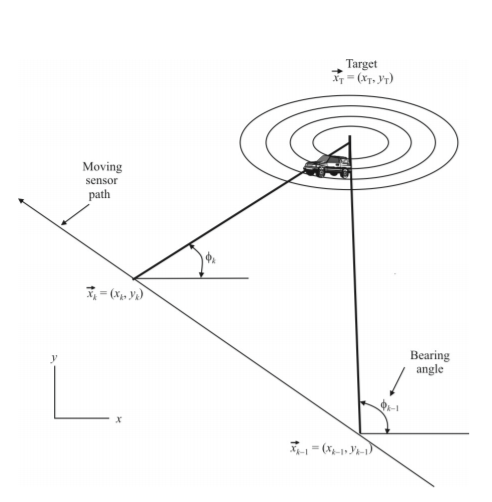
\includegraphics[width=0.5\textwidth]{target13.png}
\caption{Geometria para o Filtro de Kalman Estendido na análise do ponto fixo}
\label{target13}
\end{figure}
\end{frame}
%\begin{frame}{Exemplo}
%    \begin{figure}[ht]
%        \begin{minipage}[b]{0.32\linewidth}
%            \centering
%            \includegraphics[width = \linewidth]{example-image}
%            \caption{Label for a}
%            \label{fig:3a}
%        \end{minipage}
%        \hspace{\fill}
%        \begin{minipage}[b]{0.32\linewidth}
%            \centering
%            \includegraphics[width = \linewidth]{example-image}
%            \caption{Label for b}
%            \label{fig:3b}
%        \end{minipage}
%        \hspace{\fill}
%        \begin{minipage}[b]{0.32\linewidth}
%            \centering
%            \includegraphics[width = \linewidth]{example-image}
%            \caption{Label for c}
%            \label{fig:3c}
%        \end{minipage}
%    \end{figure}
%\end{frame}

%\begin{frame}{Exemplo}
%    \begin{figure}[ht]
%        \begin{minipage}[b]{0.49\linewidth}
%            \centering
%            \includegraphics[width = \linewidth]{example-image}
%            \caption{Label for a}
%            \label{fig:2a}
%        \end{minipage}
%        \hspace{\fill}
%        \begin{minipage}[b]{0.49\linewidth}
%            \centering
%            \includegraphics[width = \linewidth]{example-image}
%            \caption{Label for b}
%            \label{fig:2b}
%        \end{minipage}
%    \end{figure}
%\end{frame}

\begin{frame}{Referências}
  \printbibliography
\end{frame}

\end{document}